\subsubsection{Wheel Testbed Experiment 0}
\label{subsec:wheel-testbed-experiment-0}
Due to the corona pandemic, the author of this thesis did not have physical
access to research equipment until four months before the deadline of the
thesis. Nevertheless, a remote simple experiment with a
\nameref{para:single-wheel-testbed} was coordinated with the help of the
supervisor, Genya Ishigami, and other members of \SRG, namely Sora Ishikawa and
Karin Sugiura. The \nameref{para:wtb-0-data-samples} gathered in this
experiment were used in initial hypothesis testing.

\paragraph{Single Wheel Testbed}
\label{para:single-wheel-testbed}
The single wheel testbed is composed of a carriage unit attached to a frame
over a soil bin, as it can be seen in \cref{fig:single-wheel-testbed}. It is
3500 mm in length, 600 mm in width, and 1200 mm in height. The soil bin is
filled with sandy soil with a depth of 200 mm. The surface of the sand can be
leveled or sloped before each test run using the leveling apparatus attached to
the sandbox.


The carriage unit can move in the longitudinal direction at an arbitrary
velocity using the ball screw while the unit freely moves in its vertical
direction. The wheel is placed at the bottom of the carriage wheel with an
independent traction motor. Therefore this testbed can produce an arbitrary
driving condition by varying the angular speed of the wheel and the
longitudinal velocity of the unit. This driving condition is expressed as the
slip ratio $s$. The slip ratio of a smooth wheel is defined as the function of
the horizontal velocity $V_x$ and wheel angular velocity $V_\omega$ found in
\cref{eq:slip-ratio} \cite{Slip2009}, where $r$ is the radius of the wheel. The
slip ratio is bounded in the range $\left(-1,1\right]$, where negative values
correspond to wheel \emph{skidding}.

\begin{equation}
    s = \begin{cases} 
        1 - \frac{V_x}{r V_\omega} & (r V_\omega \geq V_x, 0 \leq s \leq 1) \\
        \frac{r V_\omega}{V_x} - 1 & (r V_\omega < V_x, -1 \leq s < 0)
    \end{cases} = \frac{r V_\omega - V_x}{\max(r V_\omega, V_x)}
    \label{eq:slip-ratio}
\end{equation}

This work uses the single wheel test to simplify the problem of odometry to a
straight line motion in a controlled environment. The longitudinal and vertical
movement of the wheel can be monitored by a magnetic scale, while the wheel's
angular velocity is controlled by an encoder.

Additionally, the carriage unit can be detached from the ball screw to allow
free longitudinal movement. In this way, the wheel can be driven with free slip
recreating realistic driving conditions over sandy terrain while being able to
keep accurate monitoring of its position.

Finally, the carriage unit can be loaded with additional weight in order to
recreate different driving conditions. While the experiments add different
loads, the regime of the wheel is kept under \emph{lightweight wheeled
vehicles} as defined in \cite{SENATORE2014}: average ground pressure below
20 kPa.

\paragraph{Data samples}
\label{para:wtb-0-data-samples}

During this simple remote experiment, three different wheel speeds (10, 20, and
30 deg/s) where tested with two different loads (without extra load and with an
additional 10 kg load) in free slip condition (longitudinal speed not
controlled). Additionally, the test was performed twice, with and without
contact of the wheel with the sandy terrain. The purpose of this was to
qualitatively evaluate if the wheel-terrain interaction could be appreciated in
the features extracted from the recorded audio.

\begin{figure}
    \centering
    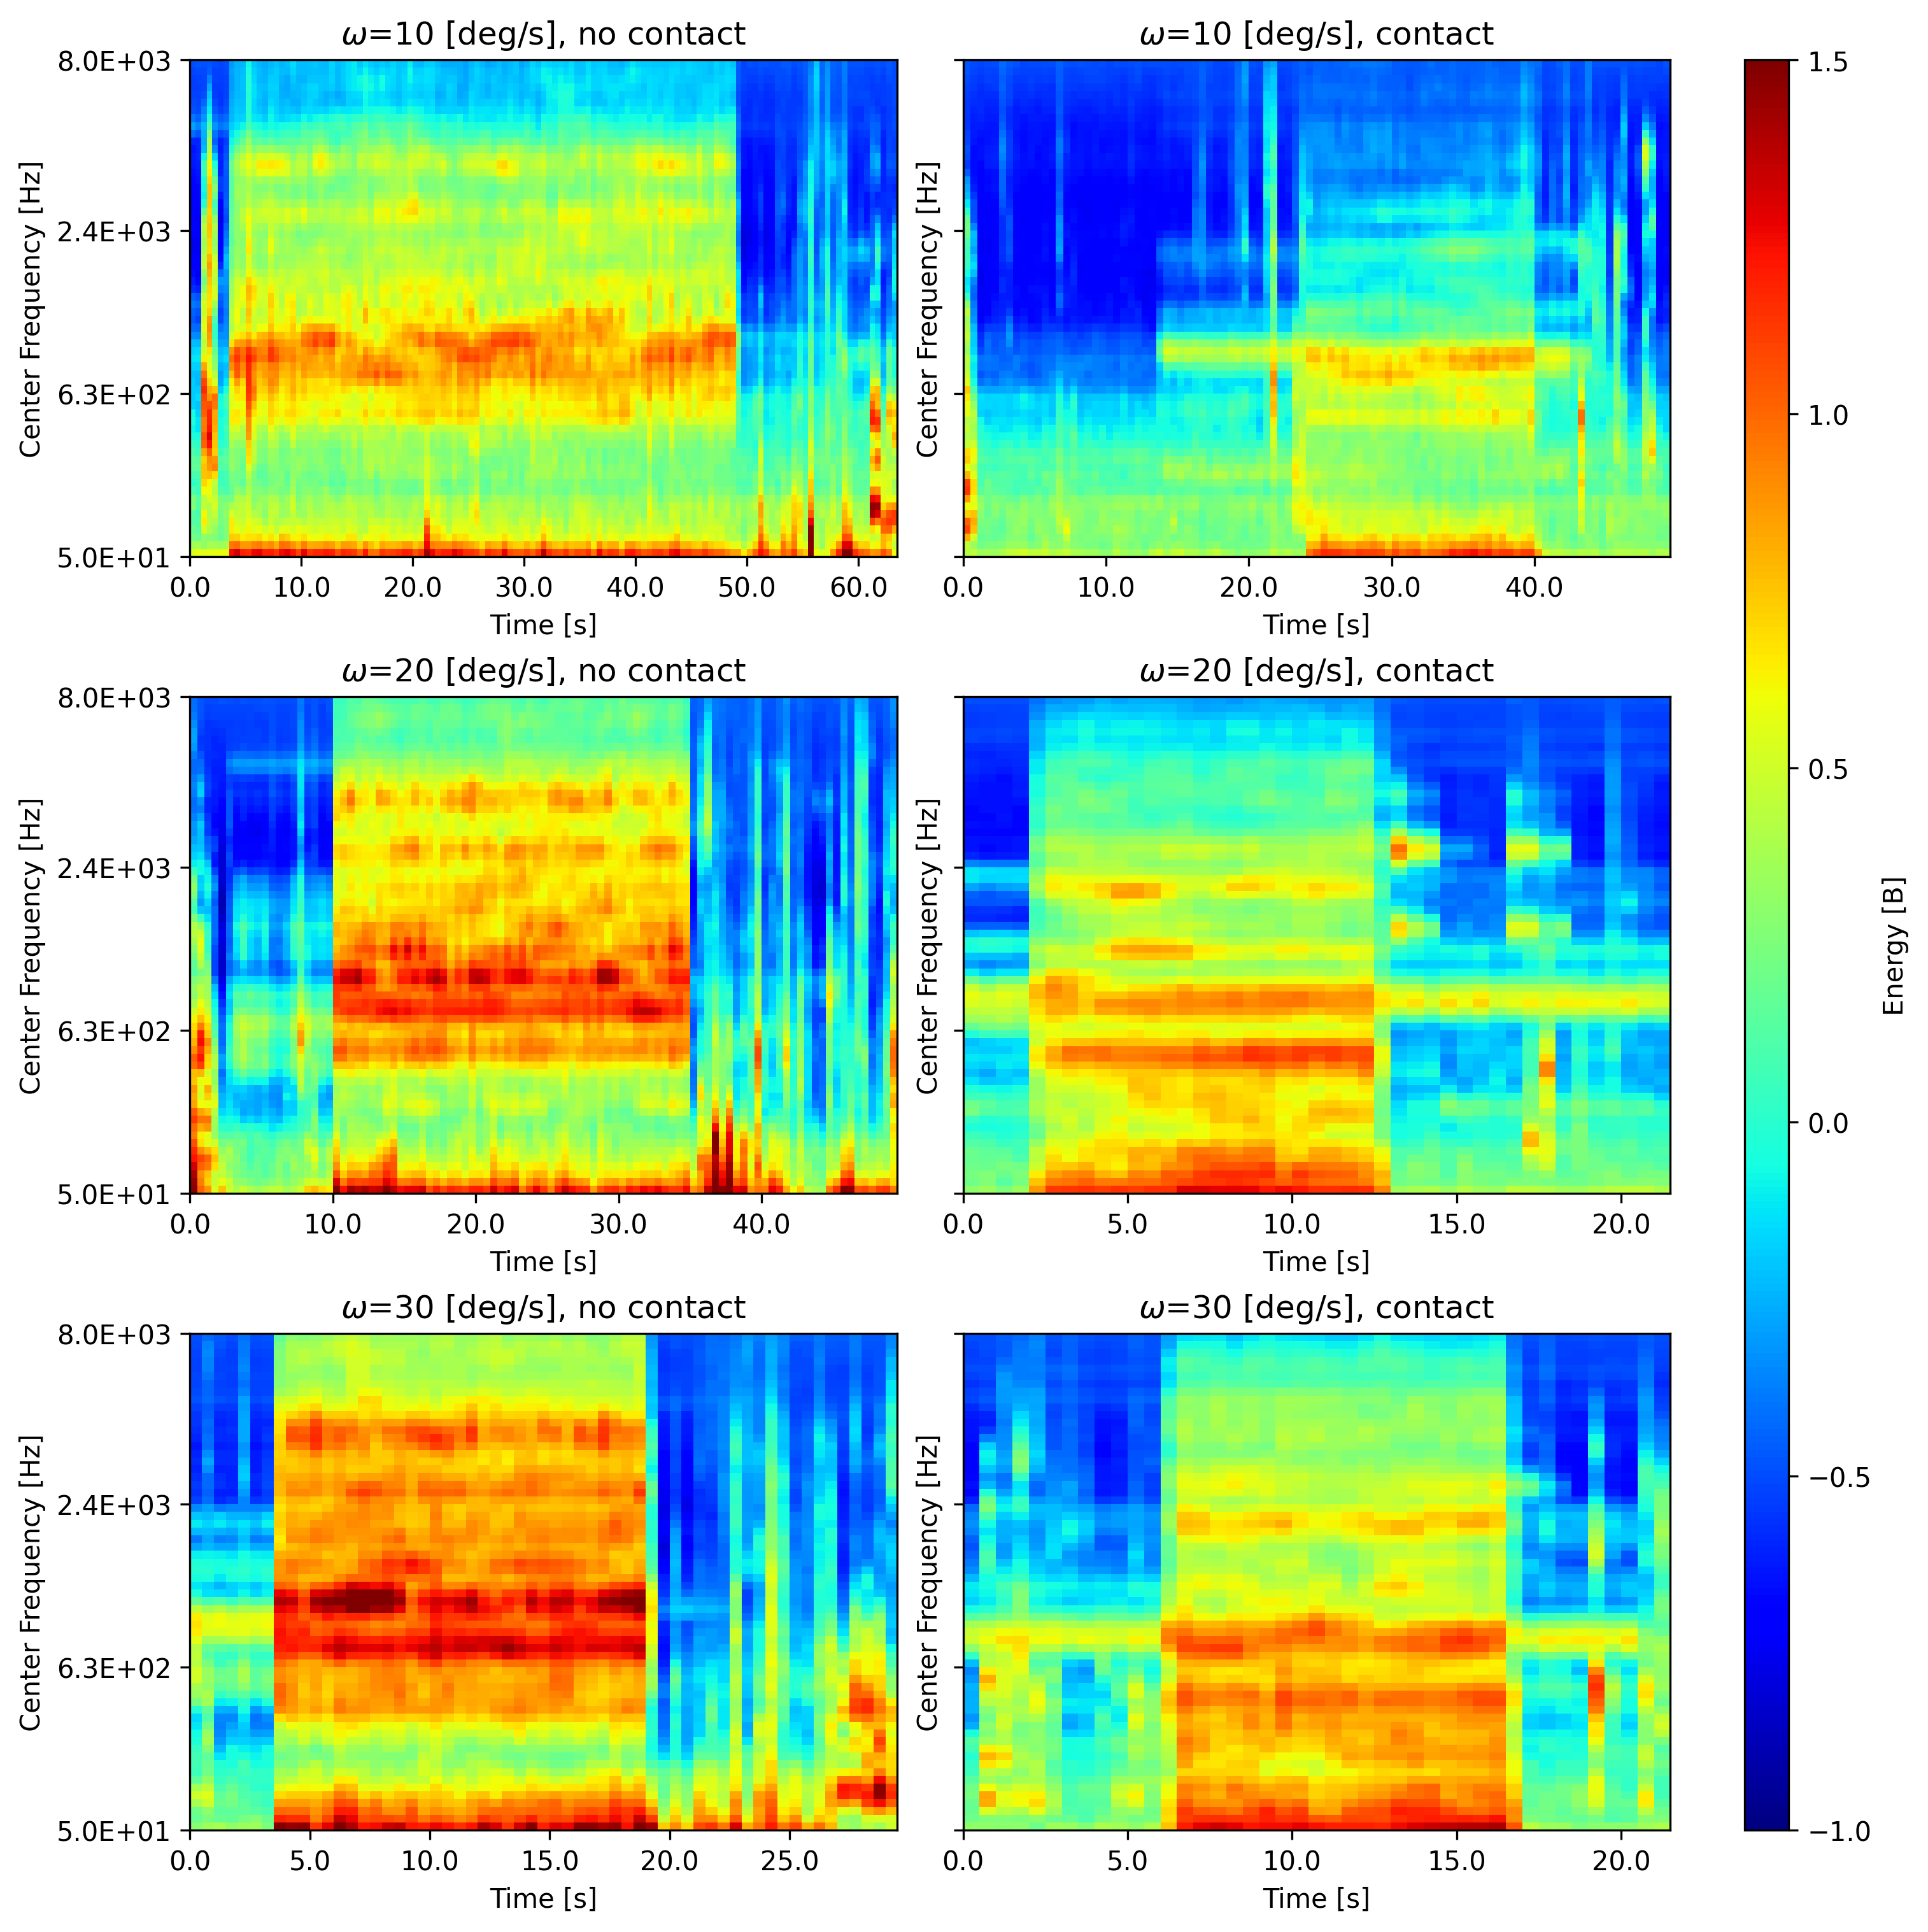
\includegraphics[width=\textwidth]{\subdir/samples.png}
    \caption[Gammatonegrams from
        \nameref{subsec:wheel-testbed-experiment-0}]{\emph{Gammatonegrams} of
        the audio recorded during different tests carried out in the
        \nameref{subsec:wheel-testbed-experiment-0}. Three driving speeds are
        shown with and without interaction between the wheel and the terrain.
        All recordings start with a period of time where the wheel does not
        move, then the wheel motor is engaged. Finally, the motor is stopped
        before the end of the audio recording.}
    \label{fig:wtb-0-data-samples}
\end{figure}


\Cref{fig:wtb-0-data-samples} shows a \emph{gammatonegram} (explained in
\cref{subsubsec:gammatone-filterbank}) of the audio recorded during the tests
in three different driving conditions, with and without wheel-terrain
interaction. One can see that the features extracted from the audio do change
when the wheel is interacting with the terrain.

However, the audio recording and the wheel movement are not orchestrated in any
way during this experiment. This can be seen in the difference between tests,
where the wheel movement duration varies considerably. This, and other issues,
are tackled in the \nameref{subsec:wheel-testbed-experiment-1} that followed
once the author of this thesis had physical access to the research equipment.
